\section{Discovery Related Articles}

In the section, we discuss the design of the framework for discovering related articles in the historical corpus. As described in section \ref{sec:3}, an article can be treated as a set of features, that are classified into \textit{meta-data} features, which consists of category, keywords, release date and length of text, and \textit{semantic} features including title, summary and content of the article. In section \ref{sec:4.1}, we discuss the motivation and the way of design the framework. In section \ref{sec:4.2}, the architecture of the framework is interpreted and it is explained, how are the components of the framework combined. In section \ref{sec:4.3} each component is explained, including preprocessing raw text, generating unsupervised features, building supervised models and update models incrementally. 

\subsection{Motivation}
\label{sec:4.1}

All STS methods and VSM models, which are introduced in section \ref{sec:2}, are applied for computing the similarity between texts. However, our goal is to find related articles of target articles. Therefore, one important problem is how different the term ``similar'' and ``related'' are, and what is the way from computing ``similarity'' to getting the ``relatedness'' degree. The terms \textit{similarity} and \textit{relatedness} are two separate concepts \cite{pedersen2007measures}. \textit{Similarity} is the measure which indicates how a text looks like another text semantically, while \textit{relatedness} is a more general concept, which contains multiple notions besides \textit{similarity}, such as causal relationship, temporal relationship and the relationship shared the same event. We explain the difference with two examples. 

\begin{description}

\item[Example 1] There are two pieces of news. One of them reports the football game of Euro Champions between FC Bayern and Real Madrid in 2014, while the other reports the football game of German Bundesliga between FC Bayern and Dortmund in 2015. Obviously, they are \textbf{similar} to each other semantically, because they share the same topic (football game) and the same subject (FC Bayern). Meanwhile, they are \textbf{unrelated} to each other. The reason is that the two games are held in the different seasons and the different competitions. Exactly, football games is quiet a kind of short-term and event-sensitive events. 

\item[Example 2] There are also two pieces of news. One reports a terrorist attack which is launched by ISIS. The other comment the war at Syria and Iraq. They are not similar, because they may share quiet a few words and meaning. However, they are related, because the both are about the consequence of ISIS. The prediction of relatedness requires knowledge of the background in this case. 

\end{description}

From the two examples, we can say that computing \textit{relatedness} is much more complicated than computing \textit{similarity}, because the machine must understand how humankind understand the identities and the differences between two articles and how to determine which are significant and which are inessential. It is thereby impossible to apply any single STS method or VSM model directly for computing \textit{relatedness} degree. From this conclusion, we design a composite framework which combines the good semantic and the meta-data features and build supervised models to utilized them. 

The motivation is derived from \cite{bar2013composite}, which researched the method to compute similarity between texts and whose system achieve took the first place of the task 6 \textit{Semantic Textual Similarity} in the SemEval2012\footnote{website: https://www.cs.york.ac.uk/semeval-2012/task6/index.php\%3Fid=results-update.html}. 

In section \ref{sec:5}, we select the set of features which represents articles in the best way and find the best combination of these features. 

\subsection{Architecture}
\label{sec:4.2}

The high-level architecture of the framework was already depicted in figure \ref{fig:highlevel}. In this section, we explain how the framework predicts related articles and improves itself. 

The whole framework can be separated sketchily into two components: unsupervised and supervised component. The unsupervised component consists of four phases of preprocessing, model building, similarity computing and model improvement. The original title, summary and content are the strings in HTML format. After preprocessing, the strings are represented as the respective sequences which the semantic models are able to deal with directly. Preprocessing contains a sub-component, called n-gram processing. N-gram processing, which converts the sequences of tokens to the sequences of phrases which contain $n$ adjacent tokens, is often applied for modeling the semantic relationship of a word with the $n-1$ predecessors. The next step is model building, which exists exclusively in the VSM models. The VSM models are built by the corpus with 

\begin{figure}[!htb]
    \centering
    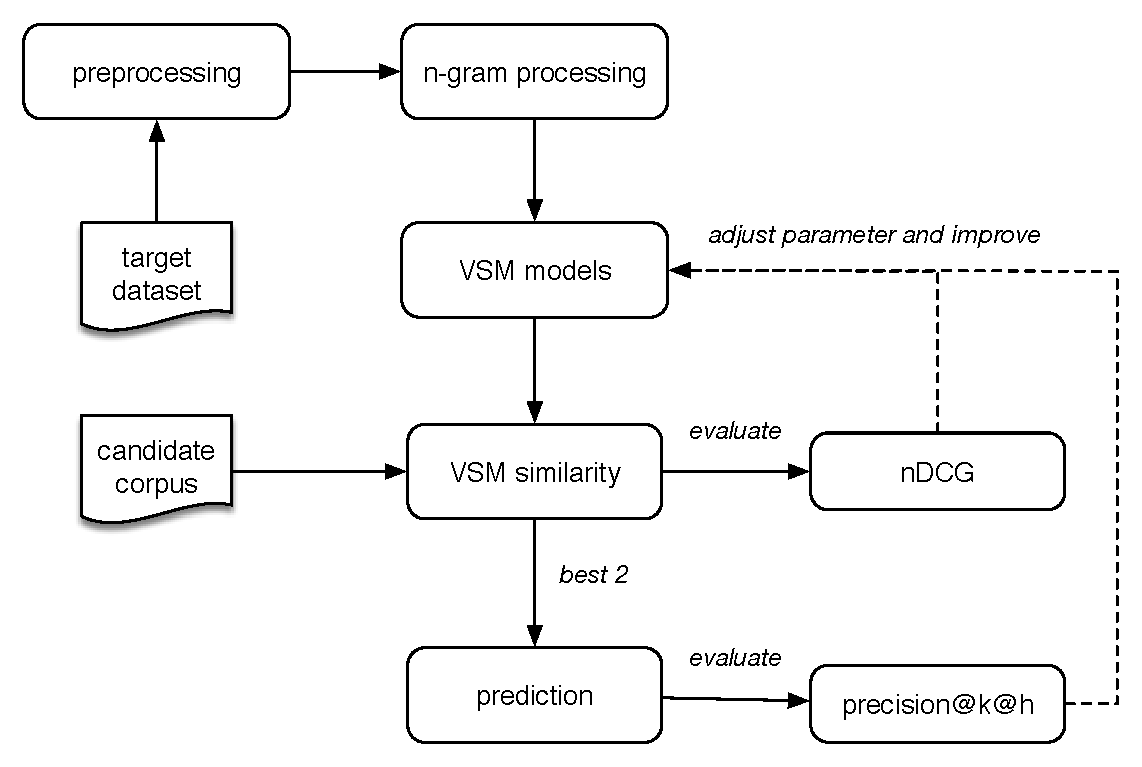
\includegraphics[width=0.7\textwidth]{fig/unsupervised}
    \caption{Caption}
    \label{fig:unsupervised}
\end{figure}

\begin{figure}[!htb]
    \centering
    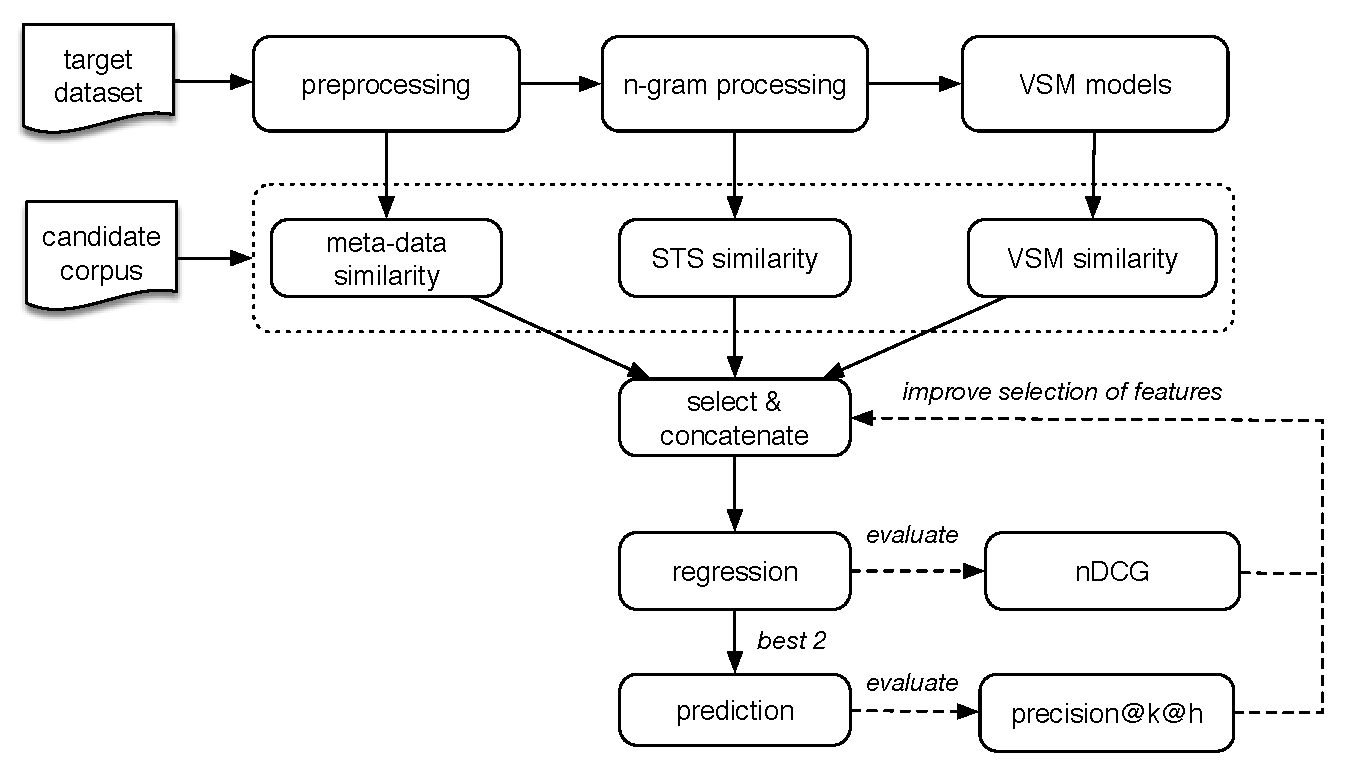
\includegraphics[width=0.85\textwidth]{fig/supervised}
    \caption{Caption}
    \label{fig:supervised}
\end{figure}

\subsection{Features and Supervised Models}
\label{sec:4.3}
\subsubsection{Meta-data Features}
\begin{description}
\item[Category] 
\item[Release Date] 
\item[Keywords] 
\item[Ratio of token length] 
\item[Ratio of term length] 
\end{description}
